\documentclass[10pt, a4paper]{article}

% fuente
\usepackage[sfdefault]{FiraSans}
\usepackage[T1]{fontenc}
\renewcommand*\oldstylenums[1]{{\firaoldstyle #1}}

% estilo parrafo
\usepackage[skip=10pt plus1pt, indent=0pt]{parskip}
\usepackage[skip=10pt plus1pt, indent=0pt]{parskip}
\usepackage{setspace}
\onehalfspacing
\hyphenpenalty 100


\usepackage{graphicx} % Required for inserting images
\graphicspath{{Resources/}}
\usepackage{hyperref}
\usepackage[spanish]{babel}


\usepackage[style=numeric, sorting=none]{biblatex}
\addbibresource{bib.bib}


\title{TFG}
\author{Diego Sanz Fuertes}
\date{July 2024}

\begin{document}
\maketitle
\titlepage
\tableofcontents
\newpage

\section{Introducción y objetivos}

En este apartado se establece el contexto y la motivación del trabajo, explicando la importancia de la síntesis de hologramas digitales generados por computador y el papel del algoritmo de trazado de rayos en el proceso. También se definen los objetivos, incluyendo la creación de escenas sintéticas, la creación de un trazador de rayos clásico, su adaptación para generar hologramas y la propagación del frente de ondas para validar los resultados.

La holografía es una técnica que permite capturar y reconstruir el campo de ondas completo de la luz. \cite{Goodman:2017} La holografía digital se utiliza hoy en día para varios propósitos, entre los que se encuentran los sistemas de pantallas tridimensionales (3D) \cite{Blinder:2019}. Las pantallas 3D holográficas permiten reproducir todas las señales de profundidad visuales naturales conocidas, como la oclusión, la acomodación del ojo, la convergencia y la estereopsis \cite{Blinder:2022}. Todas las señales de profundidad pueden observarse a simple vista en las pantallas holográficas, por lo que, en teoría, pueden reproducir una representación tridimensional fiel de cualquier escena sin restricciones en cuanto al contenido de la misma.

Los hologramas a mostrar se pueden obtener capturando el frente de ondas que viene de un objeto real, proceso análogo a realizar una fotografía, o generando el holograma mediante un computador, análogo a la generación de imágenes por computador. Uno de los mayores desafíos de la generación de hologramas por computador (CGH) es generar hologramas realistas en tiempos computacionales aceptables \cite{Blinder:2019}.

En este trabajo de final de grado se implementa un trazador de rayos para generar imágenes (2D) por computador el cuál simula el comportamiento de los rayos de luz basado en la física (Physically Based Ray Tracing o PBRT, en inglés). Además se implementa un trazador de rayos para generar hologramas (3D) por computador que hace uso de la técnica de la nube de puntos. Por último, se visualizan los hologramas generados a partir de una escena virtual, tanto por simulación como en el laboratorio.

Dado que la exigencia computacional de este problema es muy alta y mucho mayor que las aplicaciones tradicionales de la computación gráfica, este proyecto propone una solución adecuada para abordar este problema que considera la arquitectura del software, los algoritmos y la alta paralelización del problema. Esta última, tanto en CPU como en GPU utilizando los lenguajes C++ y CUDA.

\section{Estado del arte}

La generación de imágenes por computador (Computer-Generated Imagery o CGI, en inglés) es un campo de la computación gráfica bien estudiado y es utilizado en una gran variedad de áreas, como el cine y los videojuegos. Consiste, en esencia, en capturar una escena virtual en un plano, para su posterior visualización.

Una de las técnicas más utilizadas en CGI es el trazado de rayos. En la literatura se pueden encontrar libros especializados que abordan tanto la teoría como la implementación con distintos niveles de profundidad. \cite{Shirley:2024} \cite{Pharr:2023}.

El trazado de rayos (o ray tracing, en inglés) es una técnica para simular el comportamiento de la luz para sintetizar escenas virtuales. Se considera una técnica computacionalmente costosa, por lo que es utilizada principalmente para renderización offline (no en tiempo real).

Un trazador de rayos completo ha de simular al menos los siguientes objetos y fenómenos \cite{Pharr:2023}: 

\begin{enumerate}
\item Cámaras: El modelo de una cámara determina cómo y desde dónde la escena es observada, incluyendo como una imagen de la escena es recogida por un sensor.
\item Intersecciones rayo-objeto: Es necesario conocer precisamente cuándo y dónde un rayo intersecta un objeto geométrico, además de determinar algunas propiedades del objeto en el punto de intersección.
\item Fuentes de luz: El trazador de rayos ha de modelar la distribución de la luz en la escena.
\item Visibilidad: Se debe poder conocer si una luz determinada deposita energía en un punto de una superficie.
\item Dispersión de la luz en superficies: Cada objeto ha de proveer información sobre como la luz interactúa con la superficie del objeto.
\item Transporte indirecto de luz: La luz puede llegar a la superficie después de rebotar o atravesar otras superficies.
\item Propagación de rayos: Se necesita conocer el comportamiento de la luz mientras atraviesa un espacio, siendo constante en el vacío.
\end{enumerate}

La generación de hologramas por computador (Computer-Generated Holography o CGH, en inglés) es una técnica que utiliza algoritmos para generar hologramas mediante la captura del frente de ondas de una escena en un plano. 

\underline{ > Se ha de tener en cuenta que la naturaleza de la luz tiene amplitud y fase... ecuación}

$$
H(x,y) = \sum\limits_{j=1}^N a_j\exp\Big(\frac{\pi i}{\lambda z_j}\big[(x-x_j)^2 + (y-y_j)^2 \big]\Big)
$$

En el estudio \cite{Blinder:2022} se ofrece una visión general del estado del arte en CGH, una clasificación de los algoritmos y diferentes técnicas de aceleración.

Entre los algoritmos clasificados se encuentran los dos que se van a utilizar en este trabajo:

\begin{itemize}
\item Nube de puntos: Esta técnica consiste en la suma de todas las funciones de dispersión de puntos (PSFs), en el plano del holograma, que emanan de una colección de puntos luminosos. Se entiende la PSF como la función que describe respuesta de un sistema de imagen a un objeto o fuente puntual. Se puede observar en la \ref{fig:nube} figura X la función de dispersión de un punto de la escena evaluada en un plano. Las principales limitaciones de esta técnica son (1) la falta de soporte de efectos básicos como la oclusión y el sombreado; y (2) el alto coste computacional, aunque el algoritmo es altamente paralelizable \cite{Blinder:2021}

\begin{figure}[h]
    \centering 
    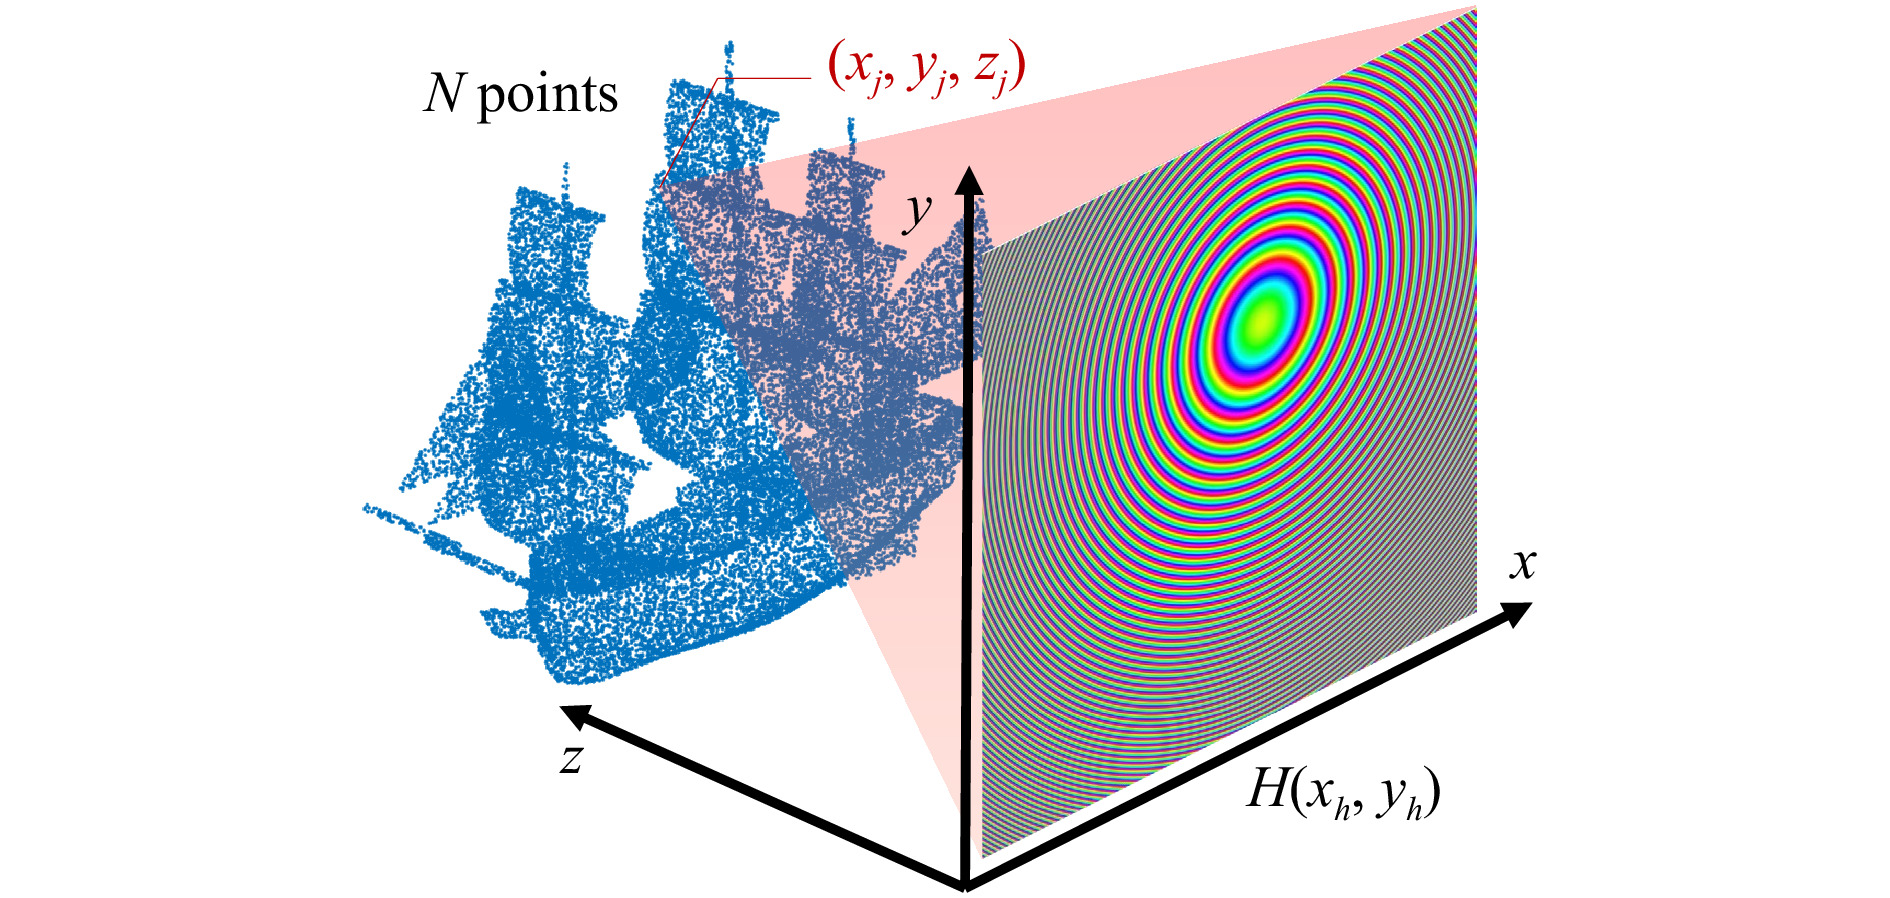
\includegraphics[width=0.75\textwidth]{tecnica_nube_puntos}

    \caption{Diagrama del algoritmo de la nube de puntos. Fuente: \textcite{Blinder:2022}.}
    \label{fig:nube}
\end{figure}

\item Trazado de rayos: Es una técnica para modelar el transporte de la luz basada en el seguimiento de rayos de luz individuales que rebotan en la escena e interactúan con materiales, calculando con precisión la cantidad de luz alcanzando cada píxel de la cámara virtual. Esta técnica puede aprovecharse en CGH para modelar también el transporte de la luz. Sin embargo, no puede utilizarse directamente, ya que la holografía se basa fundamentalmente en ondas, lo que difiere sustancialmente de los modelos basados en rayos. Uno de los principales problemas es la necesidad de obtener un continuo de puntos de vista y otro problema es la falta de coherencia de fase de la luz. Estos dos problemas hacen que los métodos basados en el trazado de rayos han de ser adaptados o combinados con otros algoritmos para ser utilizados efectivamente \cite{Blinder:2022}.
\end{itemize}

En \cite{Blinder:2021} se propone un método híbrido que toma los mejores aspectos de los métodos de nube de puntos y del trazado de rayos. En vez de calcular directamente el campo de luz en el plano del holograma, se calcula la intensidad en cada punto de la nube de puntos de la escena mediante trazado de rayos, y se calcula la PSF con esa intensidad. De este modo se consiguen efectos de iluminación realistas, sin comprometer la coherencia de la fase, lo que da lugar a vistas continuas y señales de profundidad precisas.

La naturaleza del algoritmo de trazado de rayos permite que pueda ser acelerado mediante paralelización, ya que los rayos son independientes unos de los otros. En \cite{Blinder:2021} se paraleliza en GPUs mediante CUDA y OptiX.

\underline{ > Convolución, Reordenar y definir amplitud y fase.
}

\section{Proceso de síntesis de escenas virtuales en 3D mediante hologramas digitales}

En este apartado se detalla el proceso de síntesis, dividido en tres secciones: definición de la escena virtual, generación de hologramas digitales y reconstrucción de la escena.

La implementación se ha realizado mediante el uso de los lenguajes C++ y CUDA para la definición de la escena virtual y la generación de hologramas digitales, y Python para la reconstrucción de la escena. Las librerías utilizadas se enumeran en el anexo Repositorios.

\subsection{Definición de la escena virtual}

El primer paso para la síntesis de escenas virtuales consiste en definir la escena que se desea producir. Veamos el siguiente ejemplo:

\underline{> Imagen de ejemplo
Hablar de la interfaz
> Se ha creado una interfaz de usuario la cual permite cambiar diferentes parámetros del trazador de rayos y de la escena en tiempo de ejecución...}

\subsubsection{Geometría}

La geometría de la escena se definirá mediante primitivas definidas matemáticamente. Estas primitivas son: triángulos, definidos mediante la posición espacial de sus vértices; y esferas, definidas mediante su radio y la posición espacial de su centro. 

Utilizando la primitiva del triángulo se pueden representar mallas, definidas por una lista de triángulos. El soporte de mallas resulta muy útil ya que la mayoría de modelos 3D se encuentra en este formato. 

\subsubsection{Textura}

Una vez definida la geometría de la escena, es necesario aplicar texturas a las primitivas. Las texturas que se han utilizado no siguen el significado tradicional de imágenes bidimensionales mapeadas sobre la superficie de la geometría, si no que se emplean distintos tipos de materiales, detallados a continuación:

\begin{enumerate}
    
\item Material difuso (lambertiano): Este material dispersa la luz siguiendo una distribución independiente al ángulo de incidencia y proporcional al coseno del ángulo formado entre la normal de la superficie y la dirección de dispersión. Esta distribución viene dada por la ley del coseno de Lambert. El color y la intensidad de la luz se ven modificados por el color (o albedo) del material. Este material podría describirse como mate. En la figura X se puede apreciar el comportamiento del material difuso y en la figura X se muestra un diagrama de la reflexión difusa lambertiana.

\begin{figure}[h]
     \centering 
    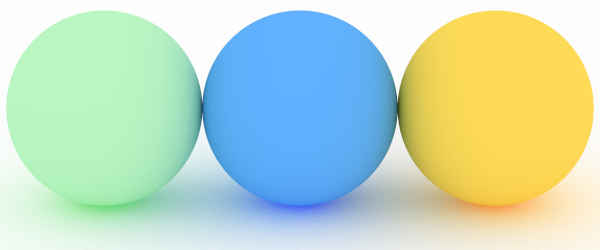
\includegraphics[width=0.75\textwidth]{02_crop}

    \caption{Render de tres esferas de diferentes colores sobre una superficie blanca. Materiales difusos.}
\end{figure}

\begin{figure}[h]
     \centering 
    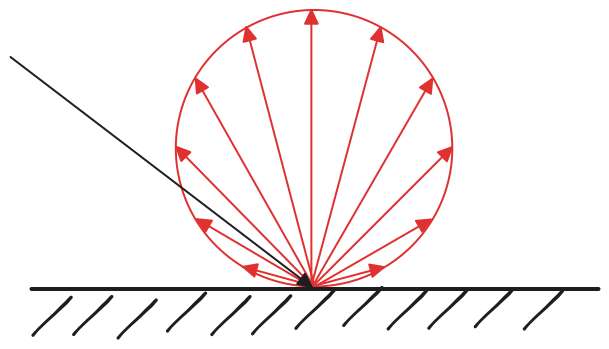
\includegraphics[width=0.75\textwidth]{lambertian}

    \caption{Diagrama de la dispersión de un material difuso lambertiano. En negro, el rayo de luz incidente, en rojo, la distribución de la dirección e intensidad de la dispersión.}
\end{figure}

\item Material metálico: Al contrario que el material difuso, el material metálico refleja la luz en el mismo ángulo en dirección opuesta respecto al ángulo de incidencia (véase figura X). Este efecto produce un reflejo de la misma manera que un espejo. Este material también cuenta con un parámetro que controla la borrosidad (o fuzziness, en inglés) del reflejo. En la figura X se puede observar el efecto espejo del material junto a el parámetro de borrosidad.

\begin{figure}[h]
     \centering 
    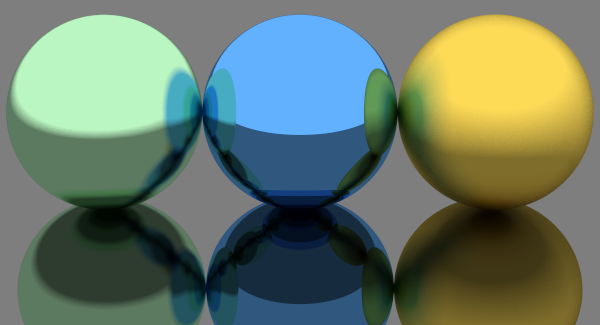
\includegraphics[width=0.75\textwidth]{03_crop}

    \caption{Render de tres esferas de diferentes colores sobre una superficie gris. Materiales metálicos con distinta borrosidad: 0.1 (izquierda), 0 (centro y superficie) y 0.5 (derecha).}
\end{figure}

\begin{figure}[h]
     \centering 
    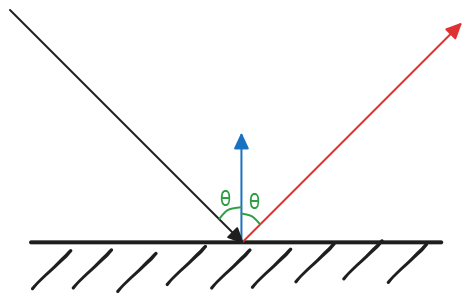
\includegraphics[width=0.75\textwidth]{metalic}

    \caption{Diagrama de la reflexión de un material metálico sin borrosidad. Rayo de incidencia en negro, rayo reflejado en rojo y vector normal a la superficie en azul.}
\end{figure}

\item Material dieléctrico: Este material representa materiales transparentes como agua y cristal. Cuando la luz incide sobre el material, se divide en luz reflejada (como el material metálico) y en luz refractada. La reflectividad se describe según las ecuaciones de Fresnel y la refracción según la ley de Snell. Este material también cuenta con un parámetro que controla el índice de refracción. En la figura X se puede apreciar el efecto de distintos índices de refracción. También se puede observar la luz refractada en la bola de la derecha debido a un índice de refracción elevado. Cabe destacar que las bolas de materiales dieléctricos no tienen sombra, se puede comprobar que ese es el caso observando una bola de cristal en un día nublado.
\end{enumerate}


\begin{figure}[h]
     \centering 
    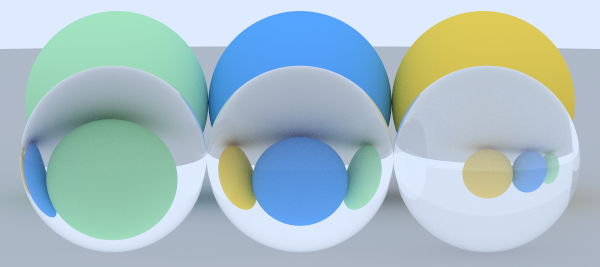
\includegraphics[width=0.75\textwidth]{04_crop}

\end{figure}

    \caption{Render de tres bolas con un material dieléctrico y tres esferas de distintos colores, sobre una superficie gris. Los indices de refracción de las tres bolas son: 1.3 (agua, izquierda), 1.5 (cristal, centro) y 2.4 (diamante, derecha).}

\begin{figure}[h]
     \centering 
    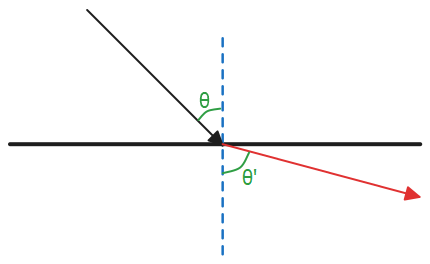
\includegraphics[width=0.75\textwidth]{dielectric}

\end{figure}

    \caption{Diagrama de la refracción de un rayo de luz al atravesar la superficie de un material dieléctrico. Rayo de incidencia en negro, rayo refractado en rojo.}

\underline{> Añadir reflejo al diagrama.}

También existen otras formas mas completas de definir materiales como las descritas en los modelos de Disney \cite{Burley:2012} o OpenPBR \cite{Academy-Software-Foundation:2024}.

\begin{figure}[h]
     \centering 
    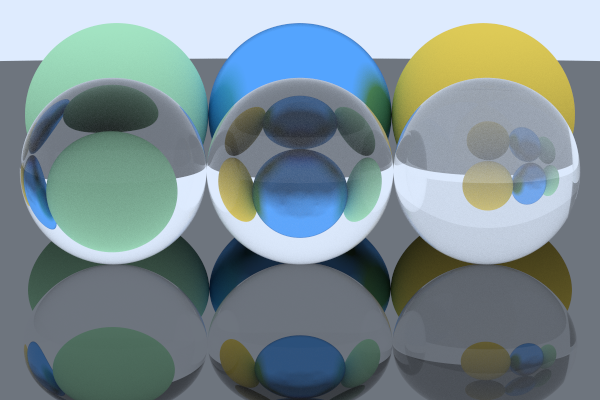
\includegraphics[width=0.75\textwidth]{01_materials}

    \caption{Render demostrando los distintos materiales. Basado en el render de la figura X (superficie y esfera azul metálicas con borrosidad 0 y 0.3 respectivamente).}
\end{figure}

\subsubsection{Iluminación}

La ultima sección de la definición de la escena virtual es la iluminación. La iluminación que se utiliza se puede dividir en dos tipos de fuente: el cielo y fuentes puntuales de luz.

El cielo ilumina de manera uniforme la escena mientras que las fuentes de luz puntuales siguen el modelo de reflexión de Blinn-Phong \cite{Blinn:1977}, que describe la forma en la que una superficie refleja la luz como una combinación de la iluminación difusa y la iluminación especular. No se incluye el término ambiental del modelo ya que se utiliza el cielo.


\begin{figure}[h]
     \centering 
    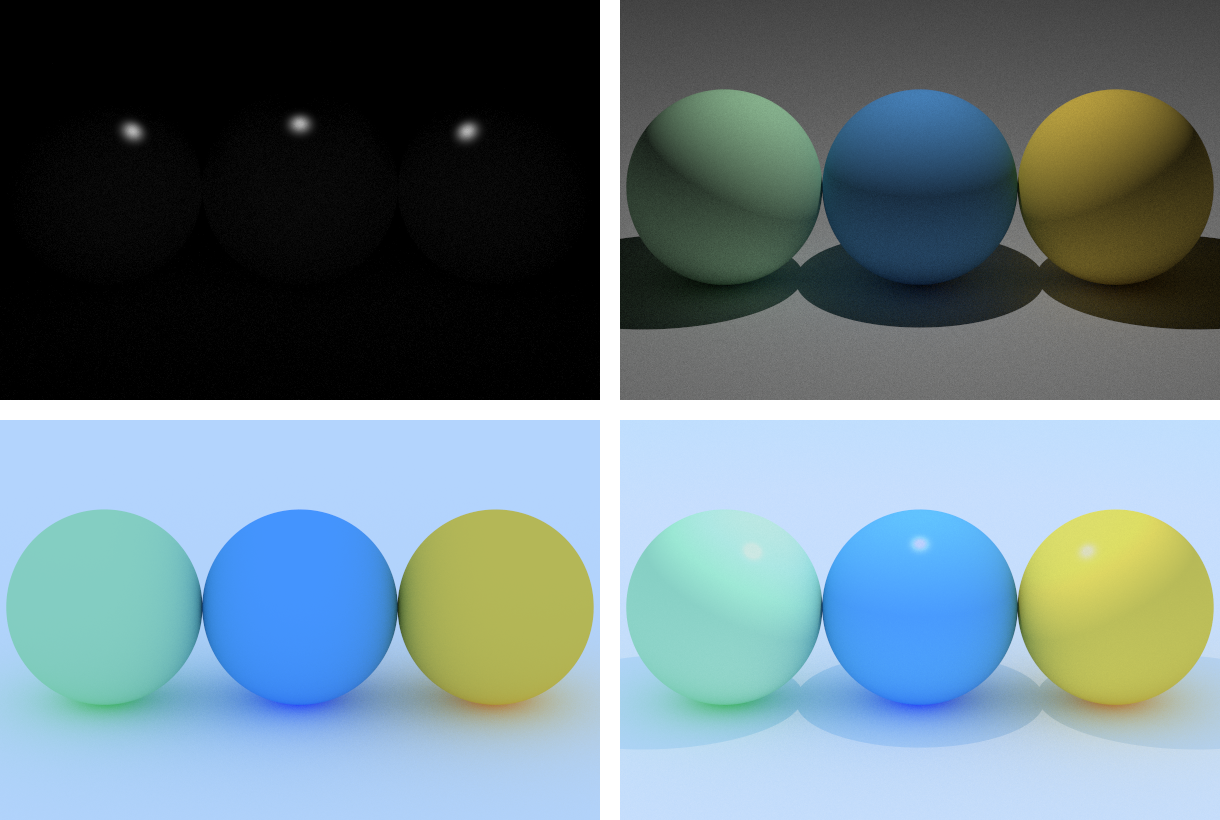
\includegraphics[width=0.75\textwidth]{05_agg}

\end{figure}

    \caption{Render de tres esferas con iluminación puntual e iluminación ambiente, separado en sus componentes: Especular (superior izquierda), difuso por punto de luz (superior derecha), difuso por iluminación ambiente (inferior izquierda) y componentes agregados (inferior derecha).}

> definición de la escena para cgh

\subsection{Generación de hologramas digitales (DH)}

\underline{> Cambiar título. Añadir introducción.}

\subsubsection{Trazado de rayos}

\underline{> En este apartado se detalla el algoritmo de trazado de rayos utilizado para generar imágenes, explicando cómo se simulan los rayos de luz desde la fuente hasta el detector y las principales diferencias con la realidad. (cámara, generación de rayos, muestreo, intersección, interacción con materiales, número máximo de rebotes, iluminación) (Referencias a los libros) (Imágenes de los resultados, la del final del primer libro y alguna malla)
> Mover a 3?}

En este trabajo concretamente se utiliza el algoritmo de trazado de caminos (o path tracing, en inglés), el cual simula más efectos que el trazado de rayos convencional gracias al uso de simulaciones de Monte Carlo (utilizando muestreo aleatorio).

\begin{figure}[h]
     \centering 
    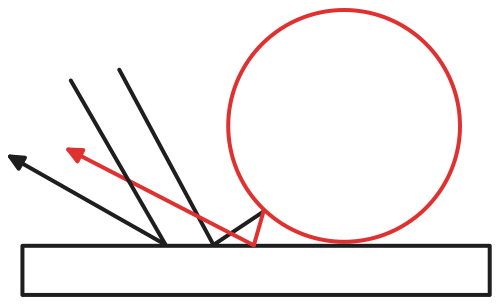
\includegraphics[width=0.75\textwidth]{bounces}

    \caption{Diagrama que muestra los posibles caminos de dos de los rayos de luz en una escena sencilla.}
\end{figure}

> poner un solo rayo

A continuación se detallará el funcionamiento de la implementación realizada en este trabajo.

\paragraph{Implementación}

Como se ha mencionado anteriormente el algoritmo se ha implementado en el lenguaje de programación C++ debido a su alto rendimiento, control sobre conceptos de bajo nivel (como gestion de la memoria) y compatibilidad con CUDA para acelerar mediante GPUs. La implementación inicial se ha basado en el libro Ray Tracing in One Weekend \cite{Shirley:2024} y se han añadido más funcionalidades no incluidas en el libro.

El primer componente del trazador de rayos es la cámara, encargada de lanzar los rayos ya que la propagación desde la fuente de luz hasta la cámara es equivalente a la propagación desde la cámara hasta la fuente de luz. La cámara se basa en una cámara estenopeica (o cámara oscura) sin lente aunque también es capaz de simular una lente para obtener el efecto de profundidad de campo.

\begin{figure}[h]
     \centering 
    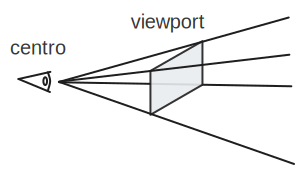
\includegraphics[width=0.75\textwidth]{camera}

\end{figure}

    \caption{Diagrama del modelo de cámara utilizado, basado en una cámara estenopeica.}

La cámara se define mediante su centro y su viewport (véase Figura X). El centro de la cámara es el punto (o el centro del disco en el caso de simular una lente) desde el cuál se originan los rayos. El viewport es un rectángulo bidimensional discretizado en píxeles utilizado para proyectar la escena. Cada píxel del viewport se corresponde con el de la imagen de salida por lo que se podría hacer un símil con el sensor de la cámara. Cada píxel indica la dirección de un rayo (véase Figura X) y una vez trazado el rayo se almacena el color resultante en la imagen de salida. Se puede obtener mayor calidad perceptual al elegir un punto aleatorio dentro del píxel en vez de su centro y se puede reducir el aliasing y aumentar la calidad al mediar el resultado de varias muestras del píxel (véase Figura X).

\begin{figure}[h]
     \centering 
    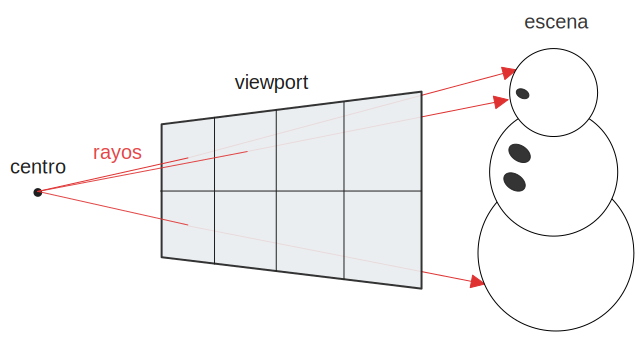
\includegraphics[width=0.75\textwidth]{camera_rays}

\end{figure}

    \caption{Diagrama del funcionamiento de la cámara en el algoritmo de trazado de rayos. Los rayos comienzan en el centro de la cámara en dirección al centro de cada pixel del viewport.}


\begin{figure}[h]
     \centering 
    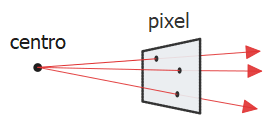
\includegraphics[width=0.75\textwidth]{camera_samples}

\end{figure}

    \caption{Diagrama del muestreo aleatorio realizado a nivel de píxel. Utilizado para reducir el aliasing y aumentar la calidad.}

Una vez lanzado el rayo se comprueba si intersecta con algún objeto de la escena iterando sobre ellos y se selecciona el objeto intersectado más cercano. De la intersección se obtiene el punto, la distancia respecto al origen del rayo, la normal de la superficie y el material del objeto. Con esta información, para la iluminación ambiente, se puede calcular la atenuación y la dirección del rayo dispersado dependiendo del material. Este proceso se repite hasta que el rayo dispersado no intersecta ningún objeto (o "escapa" de la escena) y se atenúa con el color del cielo o, si alcanza el numero máximo de rebotes definido por el trazador de rayos, la atenuación sería total. Y para la iluminación puntual, siguiendo la misma ruta del rayo de la iluminación ambiente, se comprueba si el punto es visible para la fuente de luz trazando un rayo nuevo y, si lo es, se calcula la iluminación especular y la iluminación difusa, esta última en el caso de que el material sea difuso. 


\begin{figure}[h]
     \centering 
    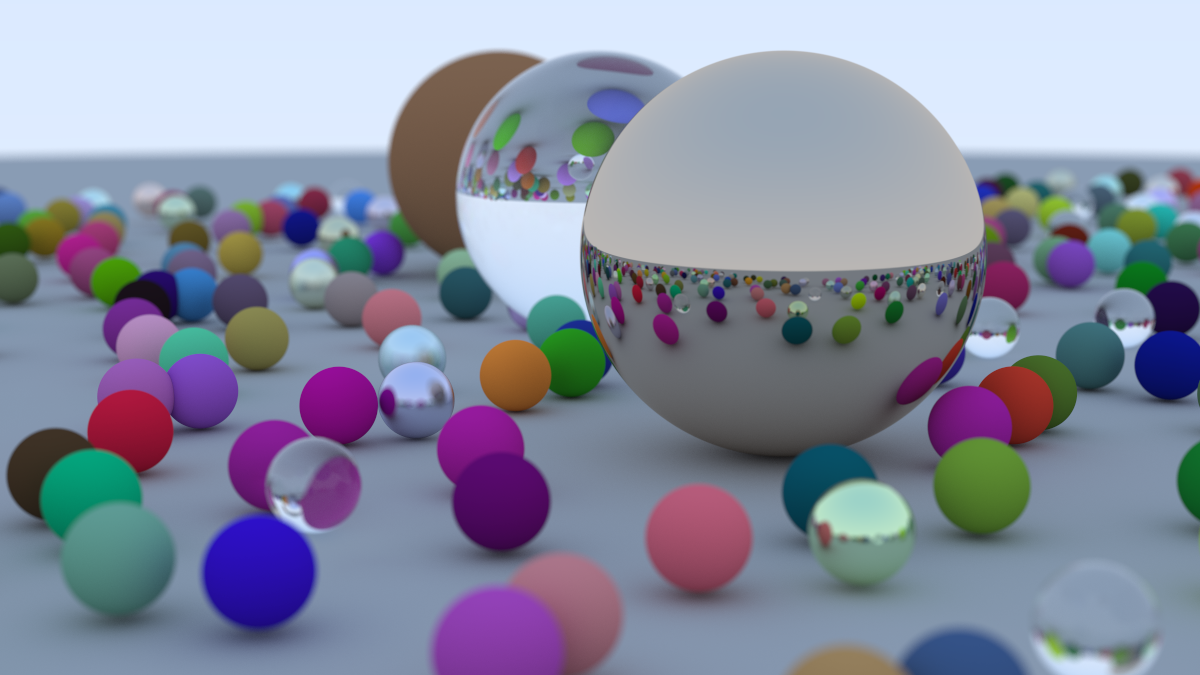
\includegraphics[width=0.75\textwidth]{06_end_book_1}
            
    \caption{Render de la escena final descrita en RTIOW.}
\end{figure}

\subsubsection{Calculo de amplitud y fase: aproximación escalar de la propagación de ondas electromagnéticas}

\underline{> En este apartado se explica el proceso de modificación del trazador de rayos descrito en el apartado anterior para el cálculo de la amplitud y la fase de las ondas electromagnéticas. (SLM, nubes de puntos, obtención de la amplitud y fase) (Referencias a los estudios) (Imágenes de los resultados, preferiblemente con poco ruido)}

Una vez implementado el trazador de rayos para la generación de imágenes, se ha modificado para generar hologramas. Las principales modificaciones realizadas han sido el proceso de lanzar rayos y el cambio del calculo del color del rayo a la amplitud y fase.

Para obtener la amplitud y la fase de cada píxel [del SLM] se ha de calcular respecto a cada punto de la escena a muestrear, siendo los mismos puntos para cada pixel por razones relacionadas con la coherencia. Para determinar estos puntos se ha utilizado la técnica de la nube de puntos, según la cual se crea una lista de puntos en las superficies de los objetos (véase Figura X). 

\begin{figure}[h]
     \centering 
    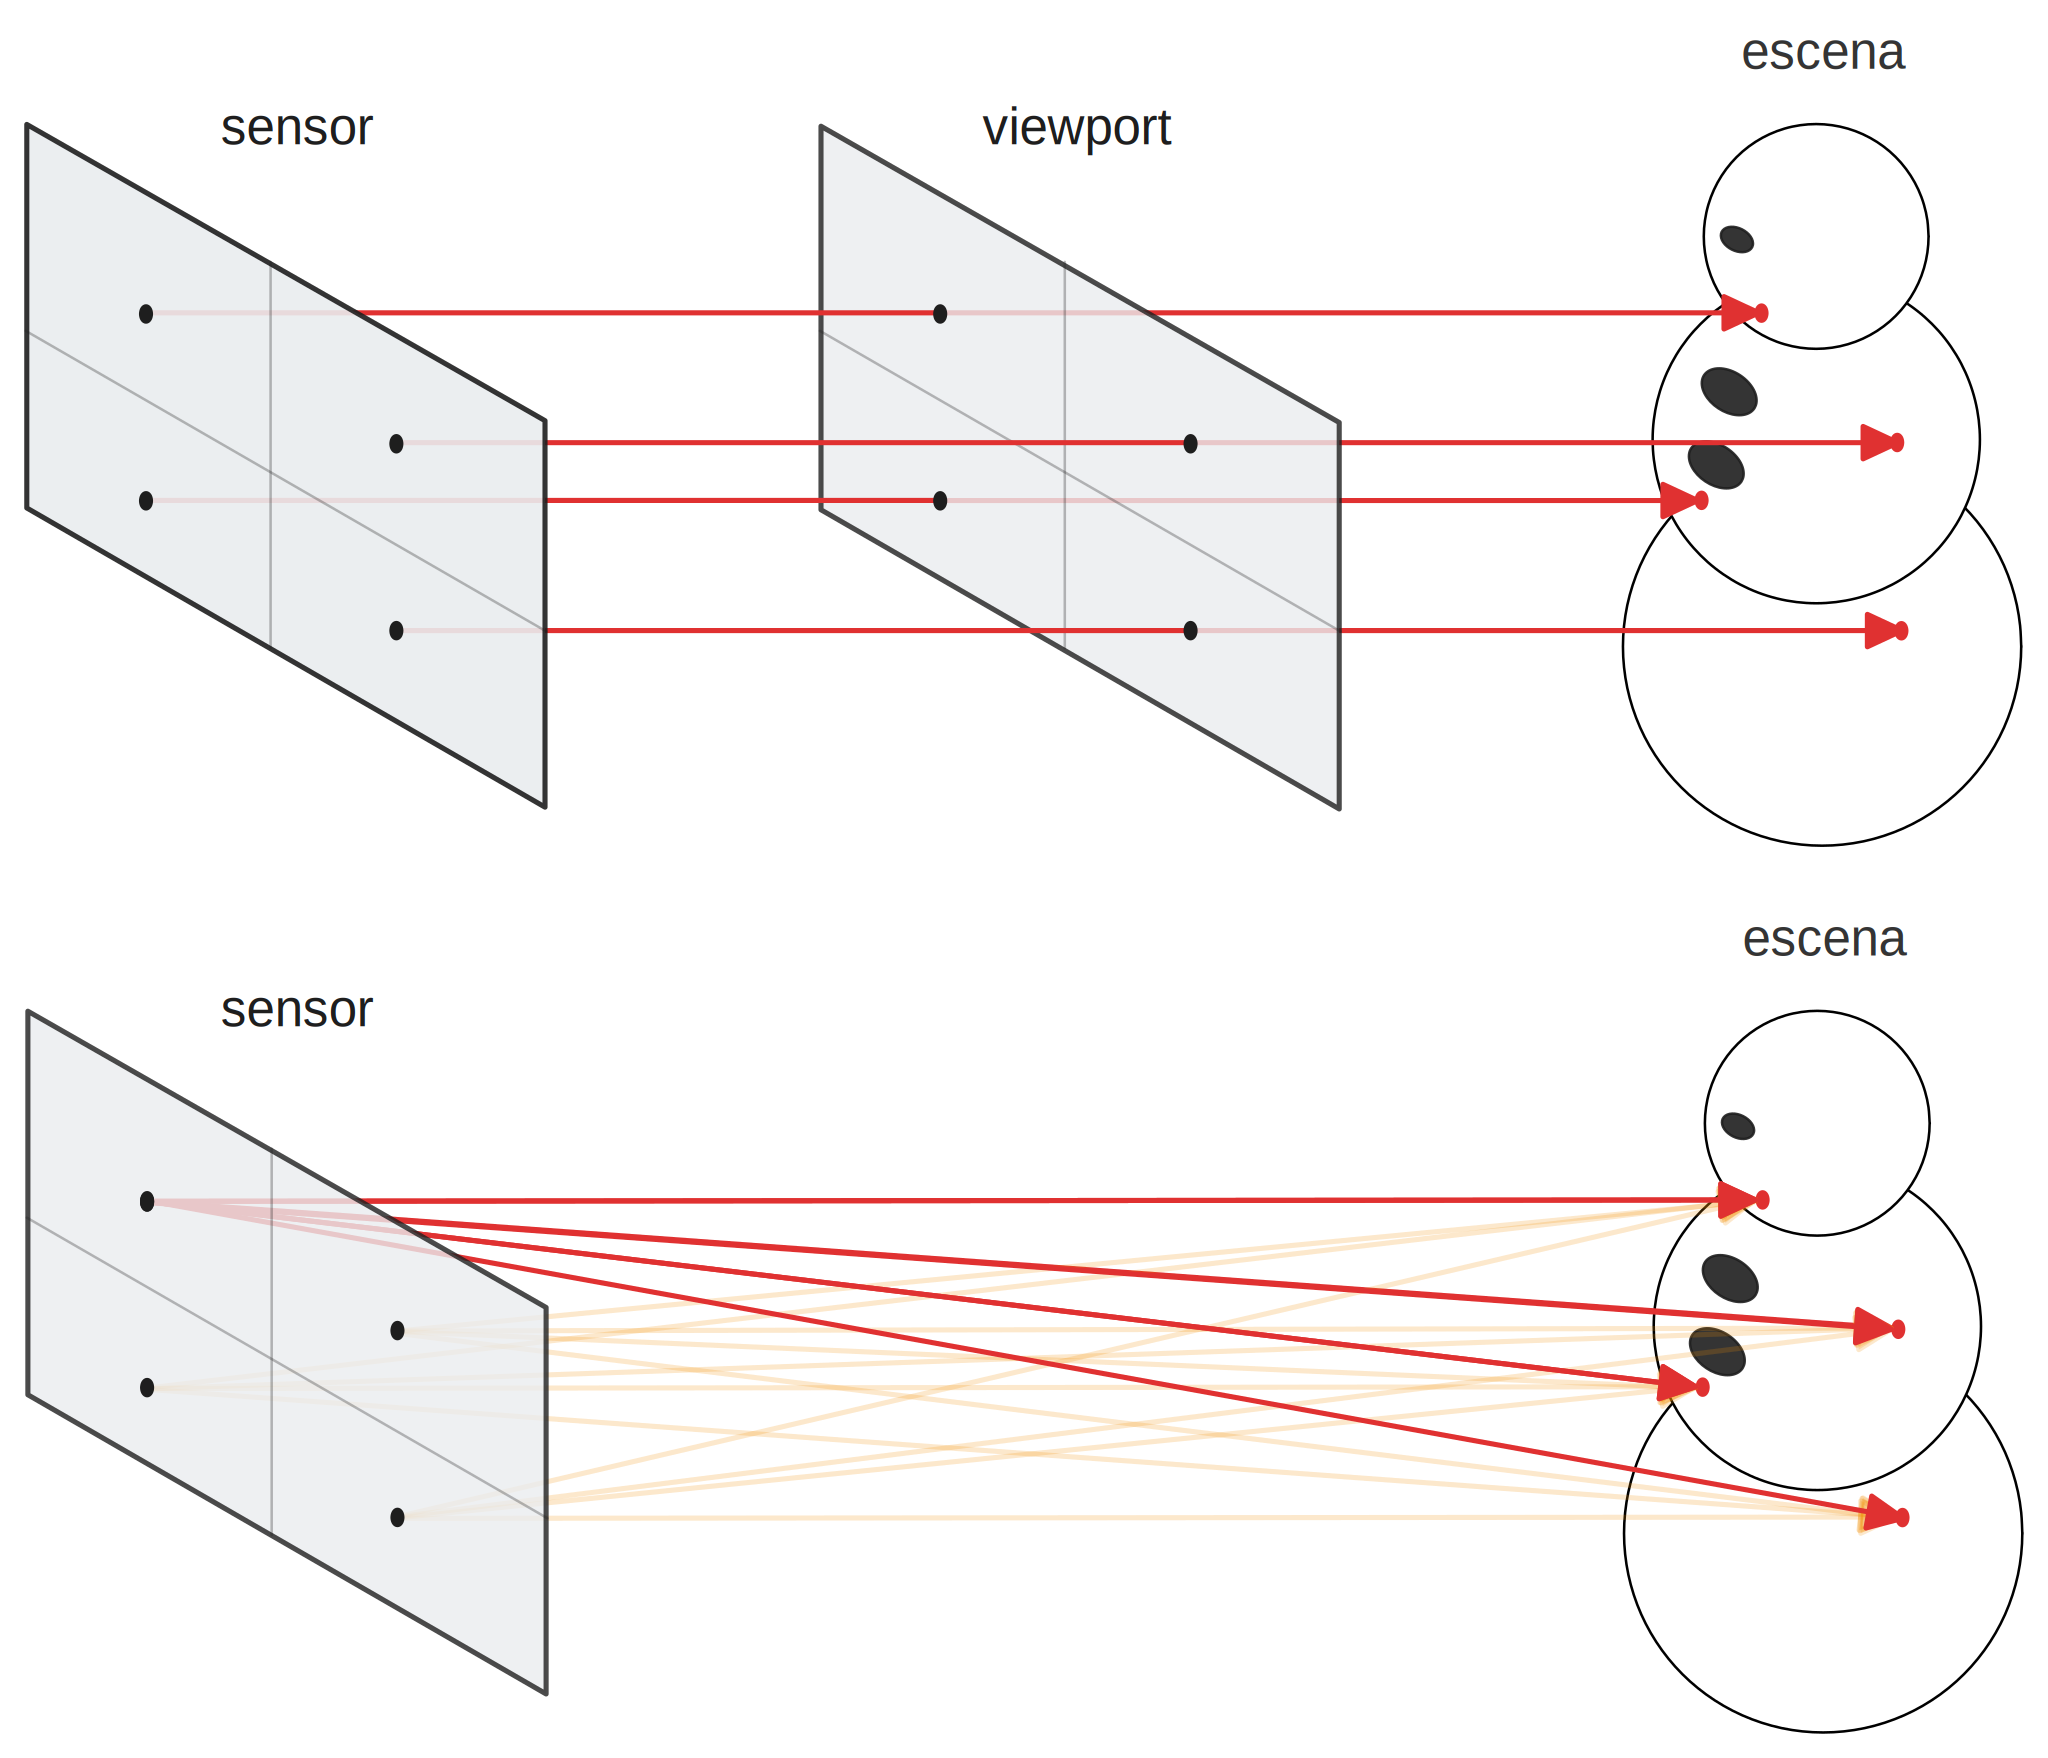
\includegraphics[width=0.75\textwidth]{slm}

\end{figure}

    \caption{Diagrama del modelo de cámara utilizado para generar hologramas. Arriba, creación de la nube de puntos; abajo, desde cada píxel del SLM se lanza un rayo en dirección a cada punto de la nube de puntos.}

\underline{> Mencionar cálculos
> Listar limitaciones respecto al CGI (dieléctricos, triángulos?, iluminación ambiental)}

\subsection{Reconstrucción de la escena}

\underline{> En este apartado se explicará brevemente el proceso de propagación de ondas electromagnéticas entre dos planos mediante convolución y el uso de las transformadas de Fourier. (Referencia al estudio) (Imágenes de los resultados a diferentes distancias)
> Quizás introducir el setup del laboratorio.}

Se han utilizado dos procesos para la reconstrucción de la escena una vez obtenido el holograma: simulación mediante la propagación de ondas electromagnéticas entre dos planos según el método de espectro angular (o angular spectrum method of plane waves, en inglés) mediante convolución en el dominio de la frecuencia y propagación en el laboratorio [gracias a un SLM y un láser]. 

La simulación se ha llevado a cabo utilizando Python como lenguaje de programación junto a la librería de computo científico NumPy.

La propagación en el laboratorio se ha realizado...

\underline{> Referencia al estudio con el kernel

> Imágenes con propagaciones a distintas distancias y comparativa entre simulación y realidad.
}

\section{Técnicas de paralelización}

La computación paralela es un tipo de computación en la que muchos cálculos o procesos se llevan a cabo simultáneamente. Existen varias técnicas de paralelización dentro de la computación paralela entre las que se encuentra la que se utilizará en este trabajo, el paralelismo de datos. Esta técnica consiste en dividir los datos entre distintos núcleos de procesamiento, los cuales operan sobre los datos en paralelo. Por ejemplo, se podría dividir una imagen en píxeles, y operar a nivel de píxel.

\subsection{CPU}

\underline{> En este apartado explicará el modelo de ejecución de las CPUs y de cómo aprovechar los diferentes núcleos mediante el uso de hilos (threads) y grupos de hilos (threadpools). (Comparación entre ambos en el caso de trazado de rayos tradicional y CGH) (Hablar de SIMD (Single Instruction Multiple Data) en algún momento o que el compilador optimiza.}

Las CPUs actuales cuentan con múltiples núcleos, lo que permite la ejecución paralela de múltiples hilos. Cada núcleo puede ejecutar una serie de instrucciones de manera independiente, permitiendo la realización de tareas en paralelo.

Para aprovechar los diferentes núcleos de la CPU es necesario dividir el trabajo para diferentes hilos (o threads, en inglés). En el caso de un trazador de rayos, el método mas sencillo de distribuir el trabajo es dividiendo la imagen en píxeles y asignando a cada hilo un rango de píxeles sobre los que operar. Este método cuenta con la limitación de que puede darse el caso de que un hilo acabe antes que otro, limitando el aumento de velocidad al hilo más lento. 

Para solucionar este problema se puede introducir el uso de un grupo de hilos (o thread pool, en inglés), al cuál se le puede asignar una serie de tareas que los hilos que lo forman ejecutan. Al dividir el trabajo en más tareas que hilos, se soluciona la limitación anterior. Se ha de tener en cuenta que la gestión de los hilos y las tareas tiene un coste computacional.

En el trazador de rayos implementado se ha dividido la imagen en líneas de píxeles y se ha optado por el uso de un grupo de hilos mediante la librería BS::thread_pool(https://github.com/bshoshany/thread-pool). La elección se debe principalmente a que el primer hilo suele terminar mucho antes que el último ya que en la mayoría de las escenas no se incluyen objetos en la parte superior. Esto no ocurre en el caso del trazador de rayos modificado para generar hologramas, ya que cada píxel lanza un rayo a cada punto y los hilos terminan con menor varianza. Por este motivo y por el coste extra del grupo de hilos, se ha optado por el uso de hilos en la generación de hologramas.

\subsection{GPU}

\underline{> En este apartado se explicará el modelo de ejecución de las GPUs junto con las distintas formas de comunicarse con la GPU (shaders, OpenCL, CUDA, otros lenguajes), centrándose en la utilización de CUDA y sus limitaciones. (diferencia código y memoria host/device, limitación a tarjetas Nvidia) (Referencia a tabla de arquitecturas CUDA) (mencionar numero de registros fp32 y fp64) (SIMD masivo)}



\section{Resultados}

\subsection{Tablas comparativas de tiempos.}

> En este apartado se detallará el hardware utilizado (CPUs y GPUs) y se realizaran comparativas entre distintas combinaciones. (CPU1 vs CPU2 vs GPU1 vs GPU2) Tanto RT como CGH (con y sin VBH (optimización Volume Binding Hierarchy)) (Diferentes resoluciones o número de puntos)

> Buscar otro nombre

\subsection{Imágenes simuladas}

> (Imágenes con más calidad, Imágenes utilizadas en el apartado anterior)

\subsection{Imágenes obtenidas en el laboratorio}

> (Comparativa entre laboratorio y simulación (CGI con blur?))

\section{Conclusiones}

\section{Trabajo futuro}

\section*{Bibliografía temporal}

- https://pbr-book.org/
- https://raytracing.github.io/
- https://developer.nvidia.com/blog/accelerated-ray-tracing-cuda/
- https://www.youtube.com/watch?v=KkOkx0FiHDA
- Computer-generated holograms for 3D imaging: A survey(https://trepo.tuni.fi//bitstream/handle/10024/127486/ACM_CSUR_Sahin_revised_submitted.pdf)

---

- https://en.wikipedia.org/wiki/General-purpose_computing_on_graphics_processing_units
- https://en.wikipedia.org/wiki/Ray_tracing_(graphics)
- https://en.wikipedia.org/wiki/Angular_spectrum_method

\printbibliography[heading=bibintoc]

\section{Anexos}

\subsection{Licencias}

\subsection{Repositorios}

\end{document}
